\vspace{10pt}

{\centering\subsection*{雷欣悦:摩擦起电}}

\addcontentsline{toc}{subsection}{雷欣悦:摩擦起电}

\renewcommand{\leftmark}{雷欣悦:摩擦起电}

\begin{figure}[htbp]

\centering

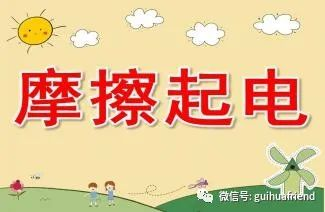
\includegraphics[width = .5\textwidth]{./ch/16.jpg}

\end{figure}





今天语文课老师带领我们做了一个实验,这个实验名称叫“摩擦起电”,因为我们都是第一次做这个实验,做第一遍的时候,我们班大多数同学都没有成功,我也在内。

就这个实验,我们要准备以下这些材料:一张纸、一把塑料尺子、一块毛面布料或者用自己的头发。

我们开始做实验,先将纸撕成一厘米大小的细纸屑,然后用塑料尺子在毛面布料或者自己的头发上摩擦一段时间,最后将摩擦过的尺子慢慢靠近纸屑上下移动,看纸屑是否跟着尺子舞动起来。

结果我第一次实验就失败了,但是我吸取了第一次的经验,第二次纸屑居然动了,我又试了一次,这一次纸屑终于吸了起来,经过两次的失败,我得出的结论就是要在毛面布料或者头发上面摩擦久一点,然后快速的靠近纸屑。

这个实验让我们懂得了,不管做什么事都不要轻易放弃。一定要大胆地去尝试,因为失败乃成功之母,你只要一次次地去尝试,就一定会成功。

今天这节课我感觉特别有意义,使我们懂得了很多道理。





\vspace{10pt}



作者:三(1)班 雷欣悦



指导老师:谢婷



投稿:2021年5月25日



发表:2021年5月26日






                



\vspace{10pt}

\hline



